\section{Overview of major embedded Linux software stacks}

\begin{frame}{D-Bus}
  \begin{columns}
    \column{0.8\textwidth}
    \begin{itemize}
    \item {\em Message-oriented middleware mechanism that allows
        communication between multiple processes running concurrently on
        the same machine}
    \item Relies on a daemon to pass messages between applications
    \item Mainly used by system daemons to offer services to client
      applications
    \item Example: a network configuration daemon, running as {\em
        root}, offers a D-Bus API that CLI and GUI clients can use to
      configure networking
    \item Several busses
      \begin{itemize}
      \item One system bus, accessible by all users, for system services
      \item One session bus for each user logged in
      \end{itemize}
    \item Object model: interfaces, objects, methods, signals
    \item \url{https://www.freedesktop.org/wiki/Software/dbus/}
    \end{itemize}
    \column{0.2\textwidth}
    \includegraphics[width=\textwidth]{slides/sysdev-software-stacks/dbus.pdf}
  \end{columns}
\end{frame}

\begin{frame}{systemd (1)}
  \begin{itemize}
  \item Modern {\em init} system used by almost all Linux
    desktop/server distributions
  \item Much more complex than {\em Busybox init}, but also much more
    powerful
  \item Only supported with {\em glibc}, not with {\em uClibc} and {\em Musl}
  \item Provides features such as
    \begin{itemize}
    \item Parallel startup of services, taking into account
      dependencies
    \item Monitoring of services
    \item On-demand startup of services, through {\em socket
        activation}
    \item Resource-management of services: CPU limits, memory limits
    \end{itemize}
  \item Configuration based on {\em unit files}
    \begin{itemize}
    \item Declarative language, instead of shell scripts used in other
      init systems
    \end{itemize}
  \end{itemize}
\end{frame}

\begin{frame}{systemd (2)}
  \begin{itemize}
  \item Systemd also provides
    \begin{itemize}
    \item {\em journald}, logging daemon, replacement for {\em syslogd}
    \item {\em networkd}, network configuration management
    \item {\em udevd}, \code{/dev} management
    \item {\em logind}, login management
    \item {\em systemctl}, tool to control/monitor systemd
    \item And many, many other things
    \end{itemize}
  \item \url{https://systemd.io/}
  \end{itemize}
\end{frame}

\begin{frame}[fragile]{systemd service unit file example}
  \begin{block}{/usr/lib/systemd/system/sshd.service}
    {
      \scriptsize
\begin{verbatim}
[Unit]
Description=OpenSSH server daemon
Documentation=man:sshd(8) man:sshd_config(5)
After=network.target sshd-keygen.service
Wants=sshd-keygen.service

[Service]
EnvironmentFile=/etc/sysconfig/sshd
ExecStart=/usr/sbin/sshd -D $OPTIONS
ExecReload=/bin/kill -HUP $MAINPID
KillMode=process
Restart=on-failure
RestartSec=42s

[Install]
WantedBy=multi-user.target
\end{verbatim}
    }
  \end{block}
\end{frame}

\begin{frame}{Example systemctl/journalctl commands}
  \begin{itemize}
  \item \code{systemctl status}, status of all services
  \item \code{systemctl status <service>}, status of one
    service
  \item \code{systemctl [start|stop] <service>}, start or stop a service
  \item \code{systemctl [enable|disable] <service>}, enable
    or disable a service, i.e. whether it should start at boot time
  \item \code{systemctl list-units}, list all available units
  \item \code{journalctl -a}, all logs
  \item \code{journalctl -f}, show the last entries, and keep printing
    new entries as they arrive
  \item \code{journalctl -u}, logs from a particular service
  \end{itemize}
\end{frame}

\begin{frame}{Linux graphics stack overview}
  \begin{center}
    \includegraphics[height=0.85\textheight]{slides/sysdev-software-stacks/graphics-stack.pdf}
  \end{center}
\end{frame}

\begin{frame}{Display controller support}
  \begin{itemize}
  \item Deprecated Linux kernel subsystem: {\em fbdev}
    \begin{itemize}
    \item Still a few old graphics drivers only available in this subsystem
    \item If possible, don't use!
    \item \url{https://en.wikipedia.org/wiki/Linux_framebuffer}
    \end{itemize}
  \item Modern Linux kernel subsystem: {\em DRM}
    \begin{itemize}
    \item Supports display controllers of SoC or graphics cards, and
      all types of display panels and bridges: parallel, LVDS, DSI,
      HDMI, DisplayPort, etc.
    \item Also supports small display panels connected over I2C or SPI
    \item Devices exposed as \code{/dev/dri/cardX}
    \item Companion user-space library: \code{libdrm}, includes a very
      handy test tool: \code{modetest}
    \item \url{https://en.wikipedia.org/wiki/Direct_Rendering_Manager}
    \end{itemize}
  \end{itemize}
\end{frame}

\begin{frame}{GPU support: OpenGL acceleration}
  \begin{itemize}
  \item Open-source
    \begin{itemize}
    \item A kernel driver in the DRM subsystem to send commands to the
      GPU and manage memory
    \item \code{mesa3d} user-space library implementing the various
      OpenGL APIs, contains massive GPU-specific logic
    \item More and more GPUs supported
    \item \url{https://www.mesa3d.org/}
    \end{itemize}
  \item Proprietary
    \begin{itemize}
    \item Many embedded GPUs used to be supported only through
      proprietary blobs $\rightarrow$ long-term maintenance issues
    \item A kernel driver provided out-of-tree by the vendor
      $\rightarrow$ they are not accepted upstream if the user-space
      is closed source
    \item A (huge) closed-source user-space binary blob implementing
      the various OpenGL APIs
    \end{itemize}
  \end{itemize}
\end{frame}

\begin{frame}{Concept of display servers}
  \begin{columns}
    \column{0.55\textwidth}
    \begin{itemize}
    \item The Linux kernel does not handle the {\em multiplexing} of the
      display and input devices between applications
      \begin{itemize}
      \item Only one user-space application can use a display and a
        given set of input devices
      \end{itemize}
    \item Display servers are special user-space applications that
      multiplex display/input by:
      \begin{itemize}
      \item Allowing multiple client GUI applications to submit their
        window contents
      \item Composing the final frame visible on the screen, based on
        contents submitted by applications, window visibility and
        layering
      \item Propagating input events to the appropriate clients, based
        on focus
      \end{itemize}
    \end{itemize}
    \column{0.45\textwidth}
    \includegraphics[width=\textwidth]{slides/sysdev-software-stacks/display-server.pdf}
  \end{columns}
\end{frame}

\begin{frame}{X11 and X.org}
  \begin{columns}[T]
    \column{0.8\textwidth}
    \begin{itemize}
    \item {\em X.org} is the historical display server on Unix
      systems, including Linux
    \item Implements the {\em X11} protocol, used between clients and
      the server
      \begin{itemize}
      \item Unix socket for local clients, TCP for remote clients
      \end{itemize}
    \item On modern Linux, works on top of DRM or fbdev for graphics,
      input subsystem for input events
    \item Still maintained, but now legacy.
    \item X11 license
    \item \url{https://www.x.org}
    \end{itemize}
    \column{0.2\textwidth}
    
\includegraphics[width=\textwidth]{slides/sysdev-software-stacks/xorg.pdf}
  \end{columns}
\end{frame}

\begin{frame}{Wayland}
  \begin{columns}[T]
    \column{0.8\textwidth}
    \begin{itemize}
    \item {\em Communication {\bf protocol} that specifies the
        communication between a display server and its clients, as
        well as a C library implementation of that protocol}
    \item A display server using the Wayland protocol is called a
      Wayland {\bf compositor}
    \item Modern replacement for the aging X11 protocol
    \item More heavily based on OpenGL technologies
    \item \url{https://wayland.freedesktop.org/}
    \item \url{https://en.wikipedia.org/wiki/Wayland_(display_server_protocol)}
    \end{itemize}
    \column{0.2\textwidth}
    
\includegraphics[width=\textwidth]{slides/sysdev-software-stacks/wayland.png}
  \end{columns}
\end{frame}

\begin{frame}{Wayland compositors}
  \begin{itemize}
  \item Weston
    \begin{itemize}
    \item The reference compositor
    \item \url{https://github.com/wayland-project/weston}
    \end{itemize}
  \item Mutter, used by the GNOME desktop environment\\
    \url{https://gitlab.gnome.org/GNOME/mutter}
  \item wlroots, a Wayland compositor library, used by
    \begin{itemize}
    \item Cage, a Wayland kiosk-style compositor\\
      \url{https://github.com/Hjdskes/cage}
    \item swayWM, a tiling Wayland compositor\\
      \url{https://swaywm.org/}
    \end{itemize}
  \item And many more\\
    \url{https://wiki.archlinux.org/title/wayland\#Compositors}
  \end{itemize}
\end{frame}

\begin{frame}{Concept of graphics toolkits}
  \begin{columns}
    \column{0.7\textwidth}
    \begin{itemize}
    \item The X11 and Wayland protocols are very low-level protocols
    \item While possible, developing applications directly using those
      protocols or their corresponding client libraries would be painful
    \item Existence of {\em toolkits}
      \begin{itemize}
      \item Some of them work only on top of a display server: X11 or
        Wayland
      \item Some of them can work directly on top of DRM + input, for
        single full-screen applications
      \end{itemize}
    \item Widget-oriented toolkits, with APIs to create windows,
      buttons, text fields, drop-down lists, etc.
    \item Game/multimedia-oriented toolkits, with no pre-defined widget
      API
    \end{itemize}
    \column{0.3\textwidth}
    \begin{center}
      \includegraphics[height=0.8\textheight]{slides/sysdev-software-stacks/toolkit.pdf}
    \end{center}
  \end{columns}
\end{frame}

\begin{frame}{Qt}
  \begin{columns}
  \column{0.7\textwidth}
  \begin{itemize}
  \item Highly popular and well-documented development framework,
    providing:
    \begin{itemize}
    \item Core libraries: data structures, event handling, XML,
      databases, networking, etc.
    \item Graphics libraries: widgets and more
    \end{itemize}
  \item Standard API is C++, but bindings to other languages available
  \item Works as
    \begin{itemize}
    \item Single application with DRM with OpenGL, or {\em fbdev} with no acceleration
    \item Multiple applications on top of X11 or Wayland
    \end{itemize}
  \item Multiplatform: Linux, MacOS, Windows.
  \item Somewhat complex licensing, with a mix of LGPLv3, GPLv2,
    GPLv3, and an (expensive) commercial license
  \item \url{https://www.qt.io/}
  \end{itemize}
  \column{0.3\textwidth}
  
\includegraphics[width=\textwidth]{slides/sysdev-software-stacks/qt-logo.pdf}
  \end{columns}
\end{frame}

\begin{frame}{Gtk}
  \begin{columns}
    \column{0.8\textwidth}
    \begin{itemize}
    \item Toolkit used as the base for the GNOME desktop environment,
      the most popular desktop environment for Linux desktop
      distributions
    \item Composed of {\em glib} (core library), {\em pango} (text
      handling), {\em cairo} (vector graphics), {\em gtk} (widget
      library)
    \item Standard API in C, but bindings exist for many languages
    \item Requires a display server: X11 or Wayland
    \item License: LGPLv2
    \item Version 3.x the most deployed currently, 4.x is a new major
      release
    \item Multiplatform: Linux, MacOS, Windows.
    \item \url{https://www.gtk.org}
    \end{itemize}
    \column{0.2\textwidth}
    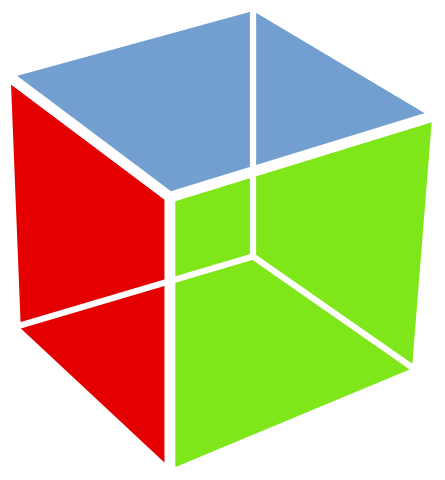
\includegraphics[width=\textwidth]{slides/sysdev-software-stacks/gtk-logo.png}
  \end{columns}
\end{frame}

\begin{frame}{Flutter}
  \begin{columns}
    \column{0.8\textwidth}
    \begin{itemize}
    \item Cross-platform UI application development: Linux, Android,
      iOS, Windows, MacOS
    \item Developed and maintained by Google
    \item Applications must be developed using the {\em Dart}
      programming language
    \item Applications can run in the Dart virtual machine, or be
      natively compiled for better performance.
    \item License: BSD-3-Clause
    \item \url{https://flutter.dev}
    \end{itemize}
    Read our blog post:
    \url{https://bootlin.com/blog/flutter-nvidia-jetson-openembedded-yocto/}
    \column{0.2\textwidth}
    % Source: https://commons.wikimedia.org/wiki/File:Google-flutter-logo.svg
    
\includegraphics[width=\textwidth]{slides/sysdev-software-stacks/Google-flutter-logo.pdf}\\
    \vspace{0.5cm}
    % Source: https://flutter.dev
    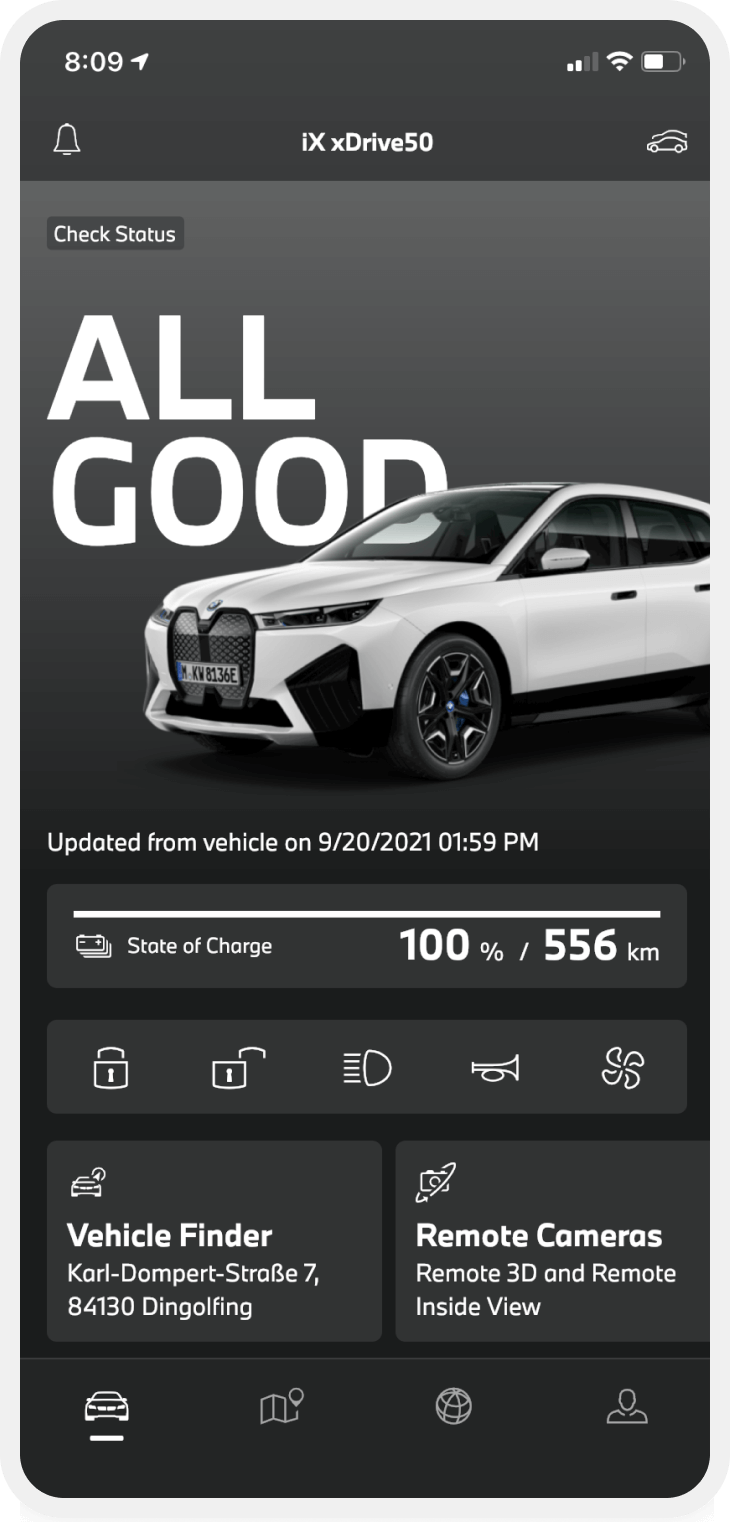
\includegraphics[width=0.9\textwidth]{slides/sysdev-software-stacks/flutter-app.png}
  \end{columns}
\end{frame}

\begin{frame}{SDL}
  \begin{columns}
    \column{0.8\textwidth}
    \begin{itemize}
    \item {\em Cross-platform development library designed to provide
        low level access to audio, keyboard, mouse, joystick, and
        graphics hardware}
    \item Implemented in C, lightweight
    \item Does not provide a widget library
    \item Games, media players, custom UIs
    \item License: zlib license (simple permissive license)
    \end{itemize}
    \column{0.2\textwidth}
    
\includegraphics[width=\textwidth]{slides/sysdev-software-stacks/sdl-logo.png}
  \end{columns}
\end{frame}

\begin{frame}{Other graphical toolkits}
  \begin{itemize}
  \item Enlightenment Foundation Libraries (EFL) / Elementary
    \begin{itemize}
    \item Lightweight and very powerful, but a lot less popular
    \item Work on top of X or Wayland.
    \item License: LGPLv2.1
    \item \url{https://www.enlightenment.org/about-efl.md}
    \end{itemize}
  \item LVGL
    \begin{itemize}
    \item Very lightweight, mostly targeted at micro-controllers, but
      also runs on Linux
    \item License: MIT
    \item \url{https://lvgl.io/}
    \end{itemize}
  \item Ensemble
    \begin{itemize}
    \item Targeted at platforms with no GPU, developed by Microchip
    \item License: Apache-2.0
    \item \url{https://ensemble.graphics/}
    \end{itemize}
  \item See \url{https://en.wikipedia.org/wiki/List_of_widget_toolkits}
  \end{itemize}
\end{frame}

\begin{frame}{Further details on Linux graphics}
  \begin{columns}
    \column{0.6\textwidth}
    \begin{itemize}
    \item Bootlin {\em Understanding the Linux graphics stack}
    \item A complete course focused exclusively on this topic
    \item Freely available training materials
    \item \url{https://bootlin.com/training/graphics}
    \end{itemize}
    \column{0.4\textwidth}
    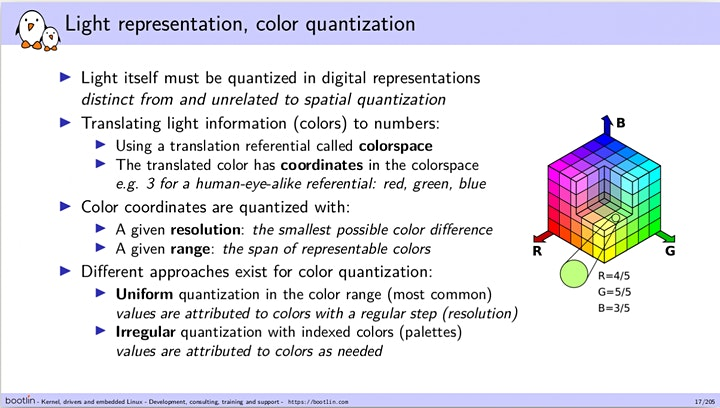
\includegraphics[width=\textwidth]{slides/sysdev-software-stacks/linux-graphics-course-slide1.jpg}
    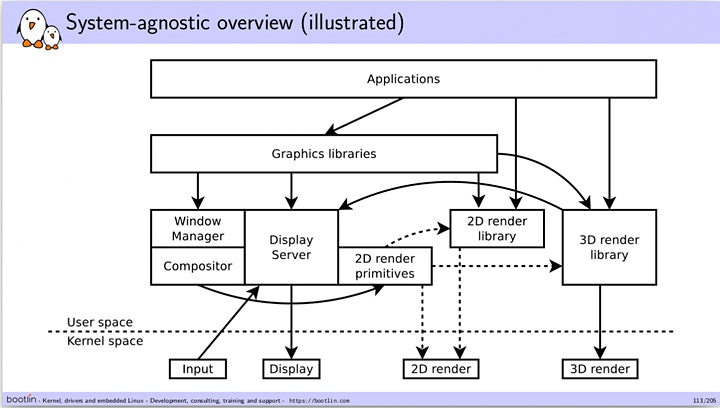
\includegraphics[width=\textwidth]{slides/sysdev-software-stacks/linux-graphics-course-slide2.jpg}
  \end{columns}
\end{frame}

\begin{frame}{Linux multimedia stack overview}
  \begin{center}
    \includegraphics[height=0.85\textheight]{slides/sysdev-software-stacks/multimedia-stack.pdf}
  \end{center}
\end{frame}

\begin{frame}{Audio stack}
  \begin{itemize}
  \item Kernel-side: the ALSA subsystem, {\em Advanced Linux Sound
      Architecture}
    \begin{itemize}
    \item Includes drivers for audio interfaces and audio codecs
    \item Exposes audio devices in \code{/dev/snd/}
    \item \url{https://alsa-project.org}
    \end{itemize}
  \item Companion user-space library: {\em alsa-lib}
  \item Audio servers
    \begin{itemize}
    \item Needed when multiple applications share audio devices: mix
      audio stream, route audio stream from specific applications to
      specific devices
    \item {\em JACK}: mainly for professional audio
    \item {\em pulseaudio}: mainly for regular desktop Linux audio
    \item {\em pipewire}: modern replacement for both pulseaudio and
      JACK, already adopted by some Linux distributions
    \item \url{https://pipewire.org/}
    \end{itemize}
  \end{itemize}
\end{frame}

\begin{frame}{Video stack}
  \begin{itemize}
  \item Kernel-side: Video4Linux subsystem, or V4L in short
    \begin{itemize}
    \item Supports camera devices: webcams as well as camera
      interfaces of SoCs and camera sensors (parallel, CSI, etc.)
    \item Also used to support video encoding/decoding HW
      accelerators: H264, H265, etc.
    \item Exposes video devices as \code{/dev/videoX}
    \item \url{https://www.linuxtv.org/}
    \end{itemize}
  \item Traditional user-space library: {\em libv4l}
  \item New user-space library, more modern, with many more features,
    under adoption: {\em libcamera}
  \item Supported in lots of multimedia stacks/software: GStreamer,
    ffmpeg, VLC, etc.
  \end{itemize}
\end{frame}

\begin{frame}{GStreamer}
  \begin{itemize}
  \item {\em Library for constructing graphs of media-handling components}
  \item Allows to create {\em pipelines} to transform, convert,
    stream, display, capture multimedia streams, both audio and video
  \item Composed of a vast amounts of plugins: video capture/display,
    audio capture/playback, encoding/decoding, scaling, filtering, and
    more.
  \item \url{https://gstreamer.freedesktop.org/}
  \item An interesting alternative is {\em ffmpeg}
  \end{itemize}

  \begin{center}
    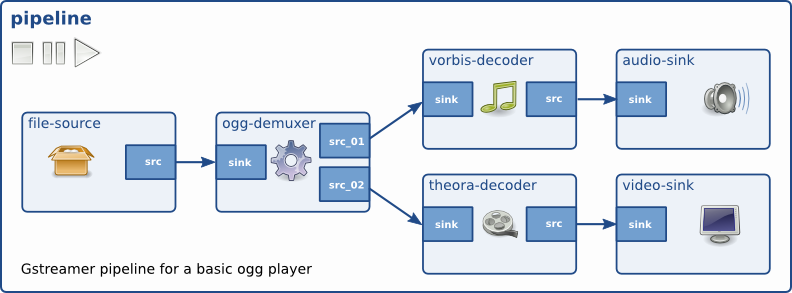
\includegraphics[width=0.6\textwidth]{slides/sysdev-software-stacks/gstreamer-pipeline.png}
  \end{center}
\end{frame}

\begin{frame}{Linux networking stack}
  \begin{center}
    \includegraphics[height=0.85\textheight]{slides/sysdev-software-stacks/networking-stack.pdf}
  \end{center}
\end{frame}

\begin{frame}{Linux connectivity stack}
  \begin{center}
    \includegraphics[height=0.7\textheight]{slides/sysdev-software-stacks/connectivity-stack.pdf}
  \end{center}
\end{frame}

\begin{frame}{Web accessible UI}
  \begin{itemize}
  \item Very common in embedded systems to use a Web interface for
    device configuration/monitoring
  \item Needs a web server: {\em Busybox httpd} for very simple needs,
    {\em lighttpd}, {\em nginx}, {\em apache} for more complex needs
  \item Can use PHP, NodeJS or other interpreted languages, or simple
    CGI shell scripts
  \end{itemize}
\end{frame}

\begin{frame}{Web browsers: rendering engines}
  \begin{itemize}
  \item WebKit
    \begin{itemize}
    \item Started by Apple, used in iOS, Safari
    \item Open source project: LGPLv2.1 and BSD-2-Clause
    \item \url{https://webkit.org/}
    \item Integrated with Gtk: \href{https://webkitgtk.org/}{WebKitGTK}
    \item Integrated with Qt: \href{https://wiki.qt.io/Qt_WebKit}{QtWebKit}
    \item Port optimized for embedded devices: \href{https://wpewebkit.org/}{WPE WebKit}
    \end{itemize}
  \item Blink
    \begin{itemize}
    \item Forked from WebKit
    \item Developed by Google, used in Chrome
    \item \url{https://en.wikipedia.org/wiki/Blink_(browser_engine)}
    \item Integrated with Qt: \href{https://wiki.qt.io/QtWebEngine}{QtWebEngine}
    \item Used by \href{https://www.electronjs.org/}{Electron}
    \end{itemize}
  \end{itemize}
\end{frame}

\begin{frame}{Web-based UIs}
  \begin{itemize}
  \item An alternative to native GUI applications is to create a GUI
    based on Web technologies
  \item Run a Web browser full-screen, and use popular Web
    technologies to develop the application
  \item Some possible options
    \begin{itemize}
    \item {\em \href{https://github.com/Igalia/cog}{Cog}},
      a simple launcher for the WPE Webkit port
    \item {\em \href{https://www.electronjs.org/}{Electron}},
      a way to package a NodeJS application with a
      web rendering engine, into a self-contained application
    \end{itemize}
  \item Beware of the footprint and performance impact: a web
    rendering engine is a massive and resource-consuming piece of
    software
  \end{itemize}
\end{frame}

\begin{frame}{Programming languages}
  \begin{itemize}
  \item Wide range of languages and frameworks available, not just C/C++
  \item Beware of footprint and performance implications
  \item Natively compiled languages
    \begin{itemize}
    \item Rust
    \item Go
    \item Ada
    \item Fortran
    \end{itemize}
  \item Interpreted languages
    \begin{itemize}
    \item Python
    \item Javascript, NodeJS
    \item Lua
    \item Shell scripts
    \item Perl, Ruby, PHP
    \end{itemize}
  \end{itemize}
\end{frame}

\setuplabframe
{Integration of additional software stacks}
{
  \begin{itemize}
  \item Integration of {\em systemd} as an init system
  \item Use {\em udev} built in {\em systemd} for automatic module
    loading
  \end{itemize}
}
